\documentclass [aspectratio=169]{beamer}
\usetheme{Boadilla}
\usepackage{textpos} % package for the positioning
\usepackage[]{graphicx}
\usepackage{graphicx}
\usepackage{float}
\usepackage{hyperref}
\usepackage{caption}
\usepackage{subcaption}
\usepackage{comment}
\usepackage{algorithm,algpseudocode}
\usepackage[export]{adjustbox}
\usepackage{tikz}
\usetikzlibrary{positioning}
\usetikzlibrary{matrix}
\usetikzlibrary{positioning}
\usetikzlibrary{arrows, shapes, decorations, automata, backgrounds, fit, petri, calc}
\newcommand{\tikzmark}[1]{\tikz[overlay,remember picture] \node (#1) {};}
\usepackage{xcolor}
\usepackage{pgfplots}

%\pgfplotsset{compat=1.10}
\usepgfplotslibrary{fillbetween}
\usepackage{filecontents}


\pgfplotsset{compat=1.7}
\usetikzlibrary{positioning}
\usetikzlibrary{arrows, shapes, decorations, automata, backgrounds, fit, petri, calc}
\setbeamertemplate{itemize items}[circle]
\setbeamertemplate{enumerate items}[circle]
\setbeamertemplate{itemize subitem}{$\triangleright$}

\newcommand{\notimplies}{\;\not\!\!\!\implies}
\newcommand*{\logofont}{\fontfamily{phv}\selectfont}
\definecolor{uoftblue}{RGB}{6,41,88} % official blue color for uoft
\definecolor{yamabuki}{RGB}{255,177,27}
\definecolor{sakuranezumi}{RGB}{177,150,147}
\definecolor{enji}{RGB}{159,53,58}
\definecolor{torinoko}{RGB}{218, 201, 166}
\definecolor{baikocha}{RGB}{137,145,107}
\definecolor{ginnezumi}{RGB}{145,152,159}


\vspace{1in}
\title[]{DoSS Summer Bootcamp Probability \\ Module 7}
\author[]{Ichiro Hashimoto}
\institute[]{University of Toronto}
\date{July 21, 2025}

% set color
\setbeamercolor{title in head/foot}{bg=white}
\setbeamercolor{author in head/foot}{bg=white}
\setbeamercolor{date in head/foot}{fg=uoftblue}
\setbeamercolor{date in head/foot}{bg=white}
\setbeamercolor{title}{fg=uoftblue}
\setbeamerfont{title}{series=\bfseries}
\setbeamercolor{frametitle}{fg=uoftblue}
\setbeamerfont{frametitle}{series=\bfseries}
\setbeamercolor*{item}{fg=uoftblue}
\setbeamercolor{block title}{bg=uoftblue}
\setbeamercolor{block title}{fg=white}
\setbeamercolor{block body}{bg=uoftblue!5!white}

% set logo at non-title pages
\logo{
\includegraphics[height=0.8cm]{logo_uoft.png}\vspace*{-.055\paperheight}\hspace*{.85\paperwidth}}

% set margin
\setbeamersize{text margin left=10mm,text margin right=10mm}

\newcommand{\mc}{\mathcal}


\begin{filecontents*}{LOFT.txt}
        n   an   a    
        1   1    0   
        2   0.5  0
        5   0.2    0   
        10   0.1    0   
        20   0.05    0   
        40   0.025    0   
        50   0.02    0   
        100   0.01    0   
\end{filecontents*}


\begin{document}
{
\setbeamertemplate{logo}{}
\begin{frame}
    \vspace{0.5in}
    \titlepage
    \begin{textblock*}{4cm}(0.5cm,-7.5cm)
        
\includegraphics[width=4cm]{logo_uoft.png}
    \end{textblock*}
    \begin{textblock*}{8cm}(5.0cm,-7cm)
        \huge \color{uoftblue}{$\Bigr\rvert$ \hspace{0.15cm} \textbf{\logofont Statistical Sciences}}
    \end{textblock*}
\end{frame}
}

\begin{frame}{Recap}
Learnt in last module:\\
\vspace{0.1in}
\begin{itemize}
    \item Covariance
    \begin{itemize}
        \item Covariance as an inner product
        \item Correlation
        \item Cauchy-Schwarz inequality
        \item Uncorrelatedness and Independence
    \end{itemize}
    \item Concentration
    \begin{itemize}
        \item Markov’s inequality
        \item Chebyshev’s inequality
        \item Chernoff bounds
    \end{itemize}
\end{itemize}
\end{frame}

\begin{frame}{Outline}
\begin{itemize}
    \item Stochastic convergence
    \begin{itemize}
        \item Convergence in distribution
        \item Convergence in probability
        \item Convergence almost surely
        \item Convergence in $L^p$
        \item Relationship between convergences
    \end{itemize}
\end{itemize}
\end{frame}


\begin{frame}{Stochastic Convergence}
    \textbf{Recall: Convergence}
    \begin{block}{Convergence of a sequence of numbers}
    A sequence $a_1, a_2, \cdots$ converges to a limit $a$ if
    $$
    \lim_{n \to \infty} a_n = a.
    $$
That is, for any $\epsilon > 0$, there exists an $N(\epsilon)$ such that
$$
|a_n - a| < \epsilon, \quad \forall n > N(\epsilon).
$$
\end{block}
\uncover<2->{
\textbf{Example: }$a_n = \frac{1}{n}$, $\forall \epsilon > 0$, take $N(\epsilon) = \lceil \frac{1}{\epsilon}\rceil$, then for $n > N(\epsilon)$,
$$
|a_n - 0| = a_n < \epsilon, \quad \lim_{n\to \infty} a_n = 0.
$$}
\end{frame}




\begin{frame}{Stochastic Convergence}
\begin{columns}
\begin{column}{0.5\textwidth}
         \begin{tikzpicture}
        \begin{axis}[xlabel=$n$, xtick={1, 10, 20, 40, 50, 100}, legend style={nodes={scale=0.8, transform shape}}, ymin = -0.05, ymax = 1.05]
        {\addplot[smooth, thick, uoftblue, mark = *, mark size = 1.5pt] table [x=n, y=an]{LOFT.txt};
        \addlegendentry{$a_n = \frac{1}{n}$}}
        {\addplot[smooth, thick, yamabuki, mark = x, mark size = 1.5pt] table [x=n, y=a]{LOFT.txt};
        \addlegendentry{$a=0$}}
        \end{axis}
        \end{tikzpicture} 
\end{column}
\begin{column}{0.5\textwidth}
\centering
\begin{itemize}
    \item Capture the property of a series as $n \to \infty$;
    \item The limit is something where the series concentrate for large $n$;
    \item $|a_n - a|$ quantifies the closeness of the series and the limit.
\end{itemize}
\end{column}
\end{columns}
\end{frame}

\begin{frame}{Stochastic Convergence}
    \textbf{Observation: closeness of random variables}\\
    \begin{block}{Sample mean of i.i.d. random variables}
    For i.i.d. random variables $X_i, i = 1, \cdots, n$ with $\mathbb{E}(X_i) = \mu$, $Var(X_i) = \sigma^2$, then for the sample mean $\bar{X} = \frac{1}{n}\sum_{i = 1}^n X_i$, 
    $$
    \mathbb{E}(\bar{X}) = \mu, \quad
    Var(\bar{X}) = \frac{\sigma^2}{n}.
    $$
    \end{block}
    \vspace{0.1in}
    \textbf{Proof:}\\
    \vspace{1in}
\end{frame}

\begin{frame}{Stochastic Convergence}
    \textbf{Example:}\\
    Further suppose $X_i, i = 1, \cdots, n$ i.i.d. with distribution $\mathcal{N}(\mu, \sigma^2)$, then $\bar{X} \sim \mathcal{N}(\mu, \frac{\sigma^2}{n})$, so we can draw the probability density plot of $\bar{X}$.\\
    \uncover<2->{
    \begin{figure}
        \centering
        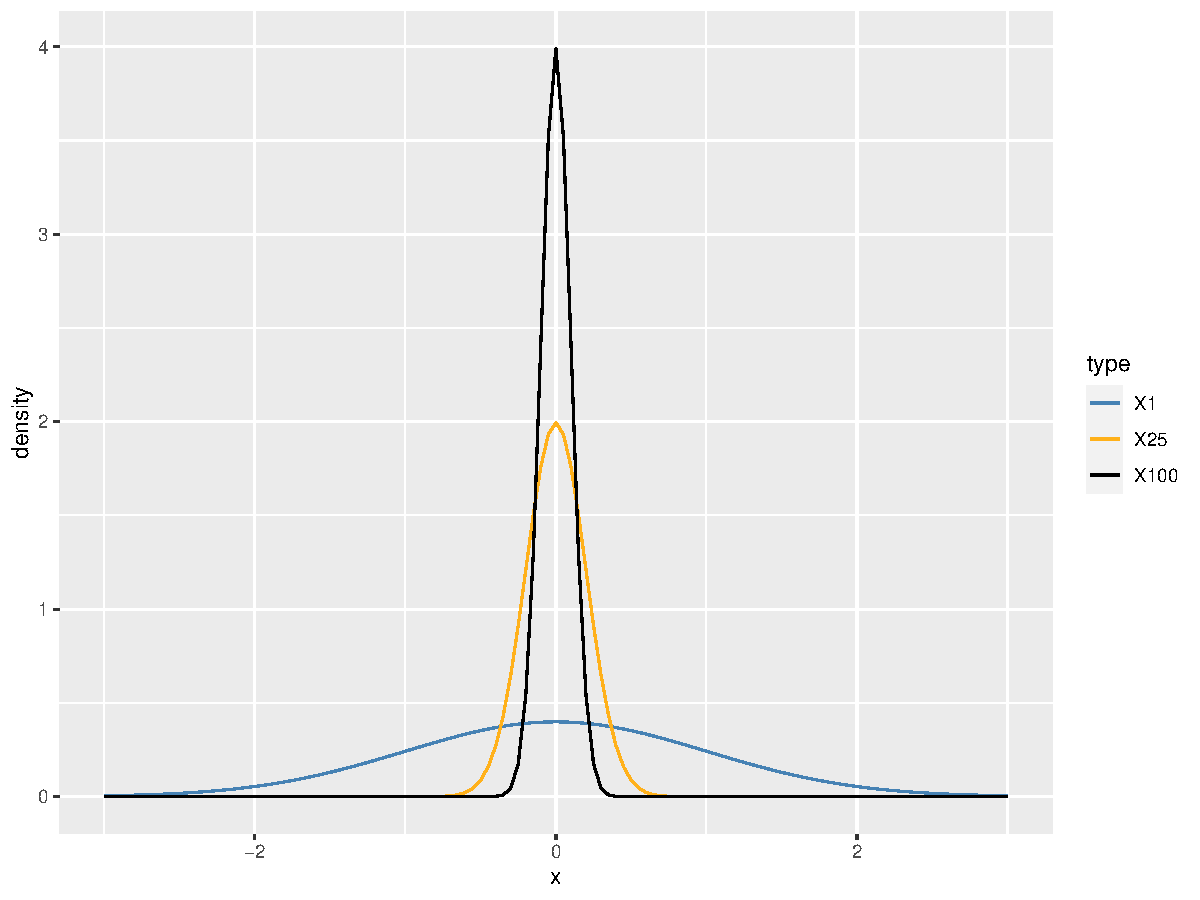
\includegraphics[width = 0.45\linewidth]{Theoretical_sample_mean.pdf}
        \caption{Probability density curve of sample mean of normal distribution}
        \label{fig:my_label}
    \end{figure}}
\end{frame}


\begin{frame}{Stochastic Convergence}
    \textbf{Intuition:}\\
    \begin{itemize}
        \item Series of numbers $a_n$ $\quad \Rightarrow \quad$ Series of random variables $X_n$;
        \item Limit $a$ $\quad \Rightarrow \quad$ Limit $X$;
        \item How to quantify the closeness? ($|X_n - X|$?)
    \end{itemize}
    \vspace{0.1in}
    \uncover<2->{
    \begin{block}{Pointwise convergence / Sure convergence}
    Suppose random variables $X_n$ and $X$ are defined over the same probability space, then we say $X_n$ converges to $X$ pointwise if
    $$
    {\displaystyle \lim _{n\to \infty }X_{n}(\omega )=X(\omega ),\,\,\forall \omega \in \Omega .}
    $$
    \end{block}}
    \uncover<3->{
    \textbf{Remark:}\\
    Incorporate probability measure in some sense. }
\end{frame}



\begin{frame}{Stochastic Convergence}
    \textbf{Alternatives of describing the closeness:}
    \begin{itemize}
        \item Utilize CDF: $F_{X_n}(x) - F_X(x)$;
        \item Utilize probability of an event: $\mathbb{P}(|X_n - X| > \epsilon)$;
        \item Utilize the probability over all $\omega$: $\mathbb{P}(\lim _{n\to \infty }X_{n}(\omega )=X(\omega))$;
        \item Utilize mean/moments: $\mathbb{E}|X_n - X|^p$.
    \end{itemize}
\end{frame}



\begin{frame}{Stochastic Convergence}
    \begin{block}{Convergence in distribution}
    A sequence $X_1, X_2, \cdots$ of real-valued random variables is said to converge in distribution, or converge weakly to a random variable $X$ if
$$
{\displaystyle \lim _{n\to \infty }F_{n}(x)=F(x),}
$$
for every number $x \in \mathbb{R}$ at which $F(\cdot)$ is continuous. Here, $F_n(\cdot)$ and $F(\cdot)$ are the cumulative distribution functions of the random variables $X_n$ and $X$, respectively.
\end{block}
\vspace{0.1in}
\textbf{Notation:}\\
$X_n \xrightarrow[]{d} X$, \quad $X_n \xrightarrow[]{\mathcal{D}} X$, \quad $X_n \Rightarrow X$. \\
\vspace{0.1in}
\uncover<2->{
\textbf{Remark:}\\
$X_n$ and $X$ do not need to be defined on the same probability space. }
\end{frame}




\begin{frame}{Stochastic Convergence}
    \textbf{Example:}\\
    Let $X_n = Z + \frac{1}{n}$, where $Z \sim \mathcal{N}(0,1)$, then 
    \begin{itemize}
        \item $X_n \xrightarrow[]{d} Z$,
        \item $X_n \xrightarrow[]{d} -Z$,
        \item $X_n \xrightarrow[]{d} Y$, $Y \sim \mathcal{N}(0,1)$.
    \end{itemize}
    \vspace{0.1in}
    \textbf{Proof:}\\
    \vspace{1in}
\end{frame}


\begin{frame}{Stochastic Convergence}
    \begin{block}{Convergence in probability}
    A sequence $X_n$ of random variables converges in probability towards the random variable $X$ if for all $\epsilon > 0$, 
    $$
    \lim _{n\to \infty }\mathbb{P} {\big (}|X_{n}-X|>\epsilon {\big )}=0.
    $$
    \end{block}
    \vspace{0.1in}
    \textbf{Notation:}
    $X_n \xrightarrow[]{p} X$, \quad $X_n \xrightarrow[]{P} X$.\\
\vspace{0.1in}
\textbf{Remark:}\\
$X_n$ and $X$ need to be defined on the same probability space. 
\end{frame}


\begin{frame}{Stochastic Convergence}
    \textbf{Examples:}\\
    \begin{itemize}
        \item Let $X_n = Z + \frac{1}{n}$, where $Z \sim \mathcal{N}(0,1)$, then $X_n \xrightarrow[]{P} Z$.\\
    \vspace{0.1in}
    \textbf{Proof:}\\
    \vspace{0.7in}
    \item Let $X_n = Z + Y_n$, where $Z \sim \mathcal{N}(0,1)$, $\mathbb{E}(|Y_n|) = \frac{1}{n}$, then $X_n \xrightarrow[]{P} Z$.\\
    \vspace{0.1in}
    \textbf{Proof:}\\
    \vspace{1in}
    \end{itemize}
\end{frame}


\begin{frame}{Stochastic convergence}
    \begin{block}{Convergence almost surely}
    A sequence $X_n$ of random variables converges almost surely or almost everywhere or with probability $1$ or strongly towards $X$ means that
$$
\mathbb{P}\left(\lim _{n\to \infty }\!X_{n}=X\right)= \mathbb{P}\left(\omega \in \Omega: \lim _{n\to \infty }\!X_{n}(\omega)=X(\omega)\right) =1.
$$
\end{block}
\vspace{0.1in}
    \textbf{Notation:}
    $X_n \xrightarrow[]{a.s.} X$.\\
\vspace{0.1in}
\textbf{Remark:}\\
$X_n$ and $X$ need to be defined on the same probability space. 
\end{frame}

\begin{frame}{Stochastic convergence}
     \textbf{Examples:}\\
    \begin{itemize}
        \item Let $X_n = Z + \frac{1}{n}$, where $Z \sim \mathcal{N}(0,1)$, then $X_n \xrightarrow[]{a.s.} Z$.\\
    \vspace{0.1in}
    \textbf{Proof:}\\
    \vspace{0.7in}
    \item Let $X_n = Z + Y_n$, where $Z \sim \mathcal{N}(0,1)$, $\mathbb{E}(|Y_n|) = \frac{1}{n}$, do we have $X_n \xrightarrow[]{a.s.} Z$?\\
    \vspace{0.1in}
    \textbf{Proof:}\\
    \vspace{1in}
    \end{itemize}
\end{frame}

\begin{frame}{Stochastic convergence}
     \begin{block}{Convergence in $L^p$}
    A sequence $\{X_n\}$ of random variables converges in $L_p$ to a random variable $X$, $p \ge 1$, if 
$$
\lim_{n \to \infty} \mathbb{E}|X_n - X|^p = 0
$$
\end{block}
\vspace{0.1in}
    \textbf{Notation:}
    $X_n \xrightarrow[]{L^p} X$.\\
\vspace{0.1in}
\textbf{Remark:}\\
$X_n$ and $X$ need to be defined on the same probability space. 
\end{frame}

\begin{frame}{Stochastic convergence}
      \textbf{Examples:}\\
    \begin{itemize}
        \item Let $X_n = Z + \frac{1}{n}$, where $Z \sim \mathcal{N}(0,1)$, then $X_n \xrightarrow[]{L^p} Z$.\\
    \vspace{0.1in}
    \textbf{Proof:}\\
    \vspace{0.7in}
    \item Let $X_n = Z + Y_n$, where $Z \sim \mathcal{N}(0,1)$, $\mathbb{E}(|Y_n|^p) = \frac{1}{n}$, then $X_n \xrightarrow[]{L^p} Z$.\\
    \vspace{0.1in}
    \textbf{Proof:}\\
    \vspace{1in}
    \end{itemize}
\end{frame}

\begin{frame}{Stochastic convergence}
    \textbf{Recall:} A random variable $X \in L^p$ if $\|X\|_{L^p} = (E |X|^p)^{1/p} < \infty$.\\ 
    \quad \qquad $X_n\to X$ in $L^p$ if $\lim_{n\to \infty}\|X_n - X\|_{L^p}=0$ \\
    \begin{block}{Monotonicity of $L^p$ Convergence}
    If $q>p>0$, $L^q$ convergence implies $L^p$ convergence 
    \end{block}
    \textbf{Proof: }
    \vspace{1.8in}
\end{frame}

\begin{frame}{Stochastic convergence}
    \textbf{Recall:} $X_n$ converges to $X$ in probability if for any $\epsilon>0$ $\lim_{n\to \infty}P(|X_n - X|>\epsilon)=0$.\\
    \begin{block}{$L^p$ convergence implies Convergence in Probability}
    If $X_n \to X$ in $L^p$, then $X_n \to X$ in probability. 
    \end{block}
    \textbf{Proof: }
    \vspace{1.8in}
\end{frame}

\begin{frame}{Stochastic convergence}
    \textbf{Recall:} $X_n$ converges to $X$ in probability if for any $\epsilon>0$ $\lim_{n\to \infty}P(|X_n - X|>\epsilon)=0$.\\
    \begin{block}{a.s. Convergence implies Convergence in Probability}
    If $X_n \to X$ almost surely, then $X_n \to X$ in probability. 
    \end{block}
    \textbf{Proof: }
    \vspace{1.8in}
\end{frame}

\begin{frame}{Stochastic convergence}
    \textbf{Recall:} $X_n$ converges to $X$ in distribution if for any continuity point $x$ of $P(X\leq x)$, $\lim_{n\to \infty}P(X_n \leq x) = P(X\leq x)$ holds.\\
    \begin{block}{Convergence in Probability implies Convergence in Distribution}
    If $X_n \to X$ in probability, then $X_n \to X$ in distribution. 
    \end{block}
    \textbf{Proof: Omitted}
    \vspace{1.8in}
\end{frame}

\begin{frame}{Stochastic convergence}
    \textbf{Relationship between convergences (on complete probability space):}\\
    \begin{figure}
        \centering
        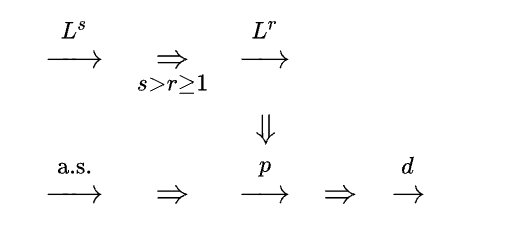
\includegraphics{convergence.png}
        \caption{relationship between convergences}
        \label{fig:my_label}
    \end{figure}
    % from wiki: https://en.wikipedia.org/wiki/Convergence_of_random_variables 
\end{frame}

\begin{frame}{Stochastic convergence}
\textbf{Highlights:}
    \begin{itemize}
        \item Almost sure convergence implies convergence in probability:
        $${\displaystyle X_{n}\ {\xrightarrow {\text{a.s.}}}\ X\quad \Rightarrow \quad X_{n}\ {\xrightarrow {\overset {}{P}}}\ X};$$
        \item Convergence in probability implies convergence in distribution:
        $$
        {\displaystyle X_{n}\ {\xrightarrow {\overset {}{P}}}\ X\quad \Rightarrow \quad X_{n}\ {\xrightarrow {\overset {}{d}}}\ X};
        $$
        \item If $X_n$ converges in distribution to a constant $c$, then $X_n$ converges in probability to $c$:
$$
X_{n}\ {\xrightarrow {\overset {}{d}}}\ c\quad \Rightarrow \quad X_{n}\ {\xrightarrow {\overset {}{P}}}\ c, \quad \text{provided $c$ is a constant}.
$$
    \end{itemize}
\end{frame}



\begin{frame}{Problem Set}
    \textbf{Problem 1:}  Prove that on a complete probability space, if $X_n  \xrightarrow[]{L^p} X$, then $X_n \xrightarrow[]{P} X$. \\
    (Hint: use Markov's inequality)\\
    \vspace{0.1in}
    
     \textbf{Problem 2:} Let $X_1, \cdots, X_n$ be i.i.d. random variables with $Bernoulli(p)$ distribution, and  $X \sim Bernoulli(p)$ is defined on the same probability space, independent with $X_i$'s. Does $X_n$ converge in probability to $X$? 
    \vspace{0.1in}\\
    
    \textbf{Problem 3:} Give an example where $X_n$ converges in distribution to $X$, but not in probability.
    \vspace{0.1in}\\
    % https://math.stackexchange.com/questions/149775/convergence-of-random-variables-in-probability-but-not-almost-surely
\end{frame}



\end{document}
